%\documentclass[Main.tex]{subfiles}
%\begin{document}

%\part{aa}

\chapter{Curvas e trajetórias}
  Neste capítulo, estudamos funções vetoriais do tipo $\vct{r}(t)$, ou seja, uma função que associa um parâmetro real a vetores no plano ou espaço. Tais função vetoriais, que dependem de apenas uma variável, são os exemplos mais simples que estudaremos. %Na seção \ref{tr}Definimos o triedro de Frenet-Serret e introduzimos os conceitos de curvatura e torção, bem como aplicações na física-matemática.

\section{Funções vetoriais de uma variável - curvas e trajetórias}
Uma função vetorial de uma variável é uma função da forma $$\vct{r}:D\to \mathbb{R}^3,$$ onde $D\subseteq \mathbb{R}$ é o domínio de definição de $\vct{r}$ e $t$ é um parâmetro - podendo ser interpretado como o tempo ou não. Em coordenadas cartesianas, uma função vetorial assume a seguinte forma:
$$\vct{r}(t)=x(t)\vct{i}+y(t)\vct{j}+z(t)\vct{k}$$
\begin{ex}\label{exfv1} São exemplos de funções vetoriais
\begin{itemize}
\item [a)] $\vct{f}(t)=\sin(t)\vct{i}+\cos(t)\vct{j}$
\item [b)] $\vct{g}(t)=t \vct{i}+\cosh(t)\vct{k}$
\item [c)] $\vct{h}(t)=2\cos(t)\vct{i}+4\sin(t)\vct{j}+t\vct{k},~~ 0\leq t \leq 8\pi$
\end{itemize}
\end{ex}  

Uma curva\index{curva} no espaço pode ser representada pelo conjunto de pontos de uma função vetorial $\vct{r}(t)$ não constante em todo o seu domínio. Um ponto $\vct{r}(t)$ de uma parametrização é dito regular se $\vct{r}\!~'(t)\neq 0$. Uma parametrização é dita regular\index{parametrização regular} em $t$ se $\vct{r}~\!'(t)\neq 0$ em todos os pontos. É possível definir orientação para uma curva regularmente parametrizada\index{orientação de uma curva}, a orientação é dada pelo sentido de crescimento do parâmetro $t$. 

\begin{ex}
A função vetorial $\vct{f}(t)=\cos(t)\vct{i}+\sin(t)\vct{j}$ para $0\leq t \leq 2\pi$ descreve  uma circunferência de raio 1 centrada na origem sobre o plano $xy$ orientada no sentido anti-horário.
\end{ex}

\begin{figure}%{0.35\textwidth}
\begin{center}
    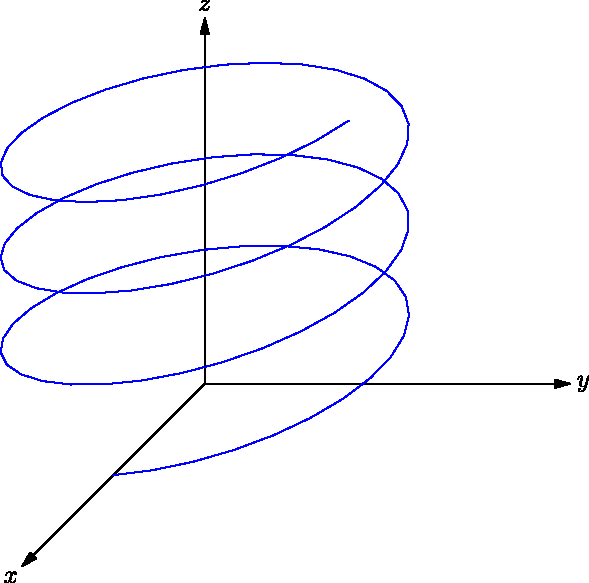
\includegraphics{./cap_curvas/pics/helice}
\caption{\label{helicedex}Hélice circular dextrogira associada à função vetorial do Exemplo~\ref{cap_curvas:exemplo_helice}.}
  \end{center}
\end{figure}

\begin{ex}\label{cap_curvas:exemplo_helice}
A função vetorial $\vct{f}(t)=\cos(t)\vct{i}+\sin(t)\vct{j}+t\vct{k}$ para $ t \in\mathbb{R}$ descreve uma hélice circular, como mostra a figura \ref{helicedex}.
\end{ex}

\begin{exer} Reconheça e represente graficamente as curvas descritas pelas seguintes funções vetoriais:
\begin{itemize}
\item [a)] $\vct{f}(t)=\sin(t)\vct{i}+\cos(t)\vct{j}+\vct{k}$, $0\leq t \leq \pi$
\item [b)] $\vct{f}(t)=\sin(t)\vct{i}+2\cos(t)\vct{k}$, $0\leq t \leq 2\pi$
\item [c)] $\vct{f}(t)=\sin(t)\vct{i}+\cos(t)\vct{k}$, $-\infty < t < \infty$
\item [d)] $\vct{f}(t)=t\vct{i}+\sqrt{4-t^2}~\!\vct{j}$, $-2 \leq t \leq 2$
\item [e)] $\vct{f}(t)=t\vct{i}+\cosh(t)\vct{j}$, $-\infty < t < \infty $
\item [f)] $\vct{f}(t)=\sinh(t)\vct{i}+\cosh(t)\vct{j}$, $-\infty < t< \infty $
\end{itemize} 
Resp: Semicircunferência de raio 1 centrada em $(0,0,1)$ sobre o plano $z=1$. Elipse de semi-eixos $1$ e $2$ centrada na origem sobre o plano $xz$. Hélice circular levogira de raio $1$ e passo $2\pi$.  Semicircunferência de raio 2 centrada na origem sobre o plano $xy$ e $y\geq 0$. Uma catenária sobre o plano $xy$. Uma hipérbole. 
\end{exer}

O limite\index{limite de uma função vetorial de uma variável}, a derivação\index{derivada de uma função vetorial de uma variável} e a integração vetorial\index{integral de uma função vetorial de uma variável} são definidas componente a componente no sistema de coordenadas cartesiano:
\begin{eqnarray}
\lim_{t\to a}\vct{r}(t)&=&\lim_{t\to a}x(t) \vct{i}+\lim_{t\to a}y(t)\vct{j}+\lim_{t\to a}z(t)\vct{k}\label{deflim}\\
\frac{d\vct{r}(t)}{dt}&=&\frac{d x(t)}{dt}\vct{i}+\frac{d y(t)}{dt}\vct{j}+\frac{d z(t)}{dt}\vct{k}\label{defder}\\
\int_{a}^b\vct{r}(t){dt}&=&\int_{a}^bx(t)dt~\!\vct{i}+\int_{a}^by(t)dt~\!\vct{j}+\int_{a}^bz(t)dt~\!\vct{k}\label{defint}\\
\int\vct{r}(t){dt}&=&\int x(t)dt~\!\vct{i}+\int y(t)dt~\!\vct{j}+\int z(t)dt~\!\vct{k}\label{defint2}
\end{eqnarray}

\begin{teo}[Regras de derivação] A derivada de funções vetoriais satisfaz as seguintes identidades:
\begin{enumerate}
\item Se $\vct{r}(t)$ é um vetor constante, então $\vct{r}'(t)=\vct{0}$. 
\item $\frac{d}{dt}\left[\alpha \vct{r}_1(t)+\beta \vct{r}_2(t)\right]=\alpha\frac{d\vct{r}_1(t)}{dt}+\beta\frac{d\vct{r}_2(t)}{dt}$
\item Se $f(t)$ é uma função real, então $\frac{d}{dt}\left[f(t) \vct{r}(t)\right]=f'(t)\vct{r}(t)+f(t)\frac{d\vct{r}(t)}{dt}$
\item $\frac{d}{dt}\left[\vct{r}_1(t)\cdot \vct{r}_2(t)\right]=\vct{r}_1(t)\cdot\frac{d\vct{r}_2(t)}{dt}+\frac{d\vct{r}_1(t)}{dt}\cdot\vct{r}_2(t)$
\item $\frac{d}{dt}\left[\vct{r}_1(t)\times \vct{r}_2(t)\right]=\vct{r}_1(t)\times\frac{d\vct{r}_2(t)}{dt}+\frac{d\vct{r}_1(t)}{dt}\times\vct{r}_2(t)$
\end{enumerate}
\end{teo}
\begin{proof} Os dois primeiros ítens podem ser obtidos diretamente de (\ref{defder}). A verificação fica a cargo do leitor. O item três pode ser obtido de  uma aplicação da regra da cadeia a (\ref{defder})\index{derivada do produto de um escalar por um vetor}:
\begin{eqnarray*}\frac{d}{dt}\left[f(t) \vct{r}(t)\right]&=& \frac{d}{dt}\left[f(t) {x}(t)\vct{i}+f(t) {y}(t)\vct{j}+f(t) {z}(t)\vct{k}\right]\\
&=&\left[f'(t) x(t)+f(t)x'(t)\right]\vct{i}+\left[f'(t) y(t)+f(t)y'(t)\right]\vct{j}+\left[f'(t) z(t)+f(t)z'(t)\right]\vct{k}\\
&=&f'(t)\left[x(t)\vct{i}+y(t)\vct{j}+z(t)\vct{k}\right]+f(t)\left[x'(t)\vct{i}+y'(t)\vct{j}+z'(t)\vct{k}\right]\\
&=&f'(t)\vct{r}(t)+f(t)\vct{r}\!~'(t)
\end{eqnarray*}

A derivada do produto escalar de duas funções vetoriais é dado por:\index{derivada do produto escalar}
\begin{eqnarray*}\frac{d}{dt}\left[\vct{r}_1(t)\cdot \vct{r}_2(t)\right]&=&\frac{d}{dt}\left[x_1(t)x_2(t)+z_1(t)z_2(t)+z_1(t)z_2(t)\right]\\
&=&
\left[x_1'(t)x_2(t)+x_1(t)x_2'(t)\right]+\left[y_1'(t)y_2(t)+y_1(t)y_2'(t)\right]
\\&+&\left[z_1'(t)z_2(t)+z_1(t)z_2'(t)\right]\\&=&\vct{r}_1(t)\cdot\frac{d\vct{r}_2(t)}{dt}+\frac{d\vct{r}_1(t)}{dt}\cdot\vct{r}_2(t)
\end{eqnarray*}
Finalmente a derivada do produto vetorial pode ser obtida de\index{derivada do produto vetorial}:
{\allowdisplaybreaks
\begin{eqnarray*}
\frac{d}{dt}\left[\vct{r}_1(t)\times \vct{r}_2(t)\right]&=&\frac{d}{dt}\left[y_1(t) z_2(t)-z_1(t)y_2(t)\right]\vct{i}\\
&+&\frac{d}{dt}\left[z_1(t) x_2(t)-x_1(t)z_2(t)\right]\vct{j}\\
&+&\frac{d}{dt}\left[x_1(t) y_2(t)-y_1(t)x_2(t)\right]\vct{k}\\
&=&\left[y_1'(t) z_2(t)+y_1(t) z_2'(t)-z_1'(t)y_2(t)-z_1(t)y_2'(t)\right]\vct{i}\\
&+&\left[z_1'(t) x_2(t)+z_1(t) x_2'(t)-x_1'(t)z_2(t)-x_1(t)z_2'(t)\right]\vct{j}\\
&+&\left[x_1'(t) y_2(t)+x_1(t) y_2'(t)-y_1'(t)x_2(t)-y_1(t)x_2'(t)\right]\vct{k}\\
&=&\left[y_1'(t) z_2(t)-z_1'(t)y_2(t)\right]\vct{i}\\
&+&\left[z_1'(t) x_2(t)-x_1'(t)z_2(t)\right]\vct{j}\\
&+&\left[x_1'(t) y_2(t)-y_1'(t)x_2(t)\right]\vct{k}\\
&+&\left[y_1(t) z_2'(t)-z_1(t)y_2'(t)\right]\vct{i}\\
&+&\left[z_1(t) x_2'(t)-x_1(t)z_2'(t)\right]\vct{j}\\
&+&\left[x_1(t) y_2'(t)-y_1(t)x_2'(t)\right]\vct{k}\\
&=&\vct{r}_1(t)\times\frac{d\vct{r}_2(t)}{dt}+\frac{d\vct{r}_1(t)}{dt}\times\vct{r}_2(t)
\end{eqnarray*}
}
\end{proof}
\begin{exer} Dada a função vetorial $\vct{r}(t)=t^2\vct{i}+e^t\vct{j}-2\cos\pi t ~\! \vct{k}$, calcule:
\begin{itemize}
\item [a)] $\displaystyle \lim_{t\to 0} \vct{r}(t)$
\item [b)] $\displaystyle \frac{d \vct{r}(t)}{dt}$
\item [c)] $\displaystyle \vct{r}~\!'(1)$
\item [d)] $\displaystyle \int_0^1 \vct{r}(t)dt$
\item [e)] $\displaystyle \int \vct{r}(t)dt$
\end{itemize}
Resp: $\vct{j}-2\vct{k}$, $\vct{r}'\!~(t)=2t\vct{i}+e^t\vct{j}+2\pi\sin\pi t ~\! \vct{k}$, $\vct{r}'\!~(1)=2\vct{i}+e\vct{j}$, $\frac{1}{3}\vct{i}+(e-1)\vct{j}$, $\left(\frac{1}{3}t^3+C_1\right)\vct{i}+\left(e^t+C_2\right)\vct{j}+\left(-\frac{2}{\pi}\sin\pi t+C_3\right)\vct{k}$

\end{exer}

\begin{exer} Verifique que a função vetorial dada por $\vct{f}(t)=\frac{1-t^2}{1+t^2}\vct{i}+\frac{2t}{1+t^2}\vct{j}$, $-\infty<t<\infty$
representa uma curva contida em uma circunferência no plano $xy$  centrada na origem. Identifique o raio desta circunferência, identifique a curva e isole os quatro quadrantes.

Resp: raio=$1$, centro na origem. $Q1: 0<t<1$, $Q2:t>1$, $Q3:t<-1$, $Q4:-1<t<0$. A curva é a circunferência menos o ponto $\left<-1,0\right>$.

\end{exer}

\begin{exer}Encontre a derivada de cada uma das funções vetoriais do exemplo \ref{exfv1}

Resp: $\vct{f'}(t)=\cos(t)\vct{i}-\sin(t)\vct{j}$,~~ $\vct{g'}(t)= \vct{i}+\sinh(t)\vct{k}$, ~~$\vct{h'}(t)=\cos(t)\vct{i}-\sin(t)\vct{j}+\vct{k}$

\end{exer}

\begin{exer} Mostre as seguintes identidades:
\begin{itemize}
\item[a)] $\displaystyle \frac{d\vct{r}(t)}{dt}\cdot \hat{r}(t)=r'(t)$
\item[b)] $\displaystyle \frac{d}{dt}\left[\vct{r}(t)\times\vct{r}~\!'(t)\right]=\vct{r}(t)\times\vct{r}~\!''(t)$
\item[c)] $\displaystyle \frac{d r(t)}{dt}=\frac{1}{r(t)} \vct{r}(t)\cdot\vct{r}~\!'(t)$
\item[d)] $\displaystyle \frac{d\hat{r}(t)}{dt}=\frac{\vct{r}~\!'(t)}{r(t)}-\frac{\vct{r}(t)\cdot\vct{r}~\!'(t)}{r(t)^3}\vct{r}(t)$
\end{itemize}
Observação: Lembre-se que $\hat{r}(t)=\frac{\vct{r}(t)}{r(t)}$ e $r(t)=\|\vct{r}(t)\|$.

\end{exer}

Demonstraremos agora um importante teorema do cálculo vetorial:
\begin{teo}\label{teodernormacst} Uma função vetorial $\vct{u}(t)$ possui norma constante se e somente se $\vct{u}(t)\cdot\vct{u}\!~'(t)=0$. 
\end{teo}
\begin{proof} Como $\|u\|^2=\vct{u}(t)\cdot\vct{u}(t)$, temos
$$\frac{d \|u\|^2}{dt}=\frac{d}{dt}\left[\vct{u}(t)\cdot\vct{u}(t)\right]=\vct{u}\cdot\frac{d\vct{u}}{dt}+\frac{d\vct{u}}{dt}\cdot\vct{u}=2\vct{u}\cdot\frac{d\vct{u}}{dt}$$
Assim, se $\|u\|$ for constante, a derivada à esquerda é nula e temos $\vct{u}(t)\cdot\vct{u}\!~'(t)=0$. Reciprocamente se $\vct{u}(t)\cdot\vct{u}\!~'(t)=0$, então $\|u\|$ deve ser constante.
\end{proof}
\begin{obs} Uma importante interpretação deste teorema é que se $\vct{v}(t)$ representa a velocidade de uma partícula no instante de tempo $t$, então se o módulo da velocidade $v(t)$ for constante e não nulo então a aceleração $\vct{a}=\vct{v}\!~'(t)$ é perpendicular à velocidade sempre que for não nula.  
\end{obs}




\begin{ex}Seja $\vct{r}(t)$ o vetor posição de uma partícula dado por
$$\vct{r}(t)=a\cos(wt)\vct{i}+a\sin(wt)\vct{j}$$
Calcule o vetor velocidade $\vct{v}$ e o vetor aceleração $\vct{v}$ dados por $\vct{v}=\vct{r}~\!'(t)$ e $\vct{a}=\vct{v}~\!'(t)$.
\end{ex}



 
 \section{Comprimento de arco}
% Dada uma curva parametrizada pela função vetorial $\vct{r}(t)=x(t)\vct{i}+y(t)\vct{j}+z(t)\vct{k}$, $t\in[a,b]$, estamos interessados no problema de calcular o comprimento $L$ do arco de descrito por uma curva $\vct{r}(t)$, $a\leq t\leq b$.
  
\begin{figure}
\centering
    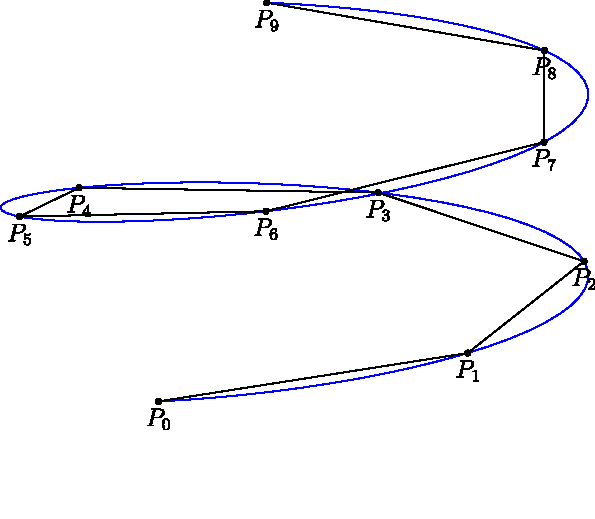
\includegraphics{./cap_curvas/pics/helice_retificacao}
\caption{Aproximação poligonal do comprimento do arco}\label{fig_compr_arc}
\end{figure}

 
 
Seja $a=t_0<t_1<t_2<\cdots<t_n=b $ uma partição equidistante do domínio com $\Delta t=t_i-t_{i-1}$ e $P_i=\vct{r}(t_i)$, $i=0,1,\cdots,n$, pontos sobre a curva, como mostra a figura \ref{fig_compr_arc}. Uma possível aproximação para o comprimento da curva é dado pelo comprimento da poligonal. Observe que o comprimento do segmento $P_{i-1}P_i$ é dado por $\|P_i-P_{i-1}\|$, logo, a aproximação para o comprimento da curva é
\begin{eqnarray*}
L_n&=&\sum_{i=1}^n\|P_i-P_{i-1}\|\\
&=&\sum_{i=1}^n \sqrt{(x_i-x_{i-1})^2+(y_i-y_{i-1})^2+(z_i-z_{i-1})^2}\\
&=&\sum_{i=1}^n \Delta t \sqrt{\frac{(x_i-x_{i-1})^2}{(\Delta t) ^2}+\frac{(y_i-y_{i-1})^2}{(\Delta t) ^2}+\frac{(z_i-z_{i-1})^2}{(\Delta t) ^2}}\\
&=&\sum_{i=1}^n \sqrt{\left(\frac{x_i-x_{i-1}}{\Delta t }\right)^2+\left(\frac{y_i-y_{i-1}}{\Delta t}\right)^2+\left(\frac{z_i-z_{i-1}}{\Delta t}\right)^2}\Delta t.
\end{eqnarray*}
Naturalmente, $L=\lim_{n\to\infty }L_n$. Como o lado direito da última igualdade é uma soma de Riemann, temos:
\begin{equation}\label{defcomparco}
L=\bigintss_{a}^{b} \sqrt{\left(\frac{dx(t)}{dt}\right)^2+\left(\frac{dy(t)}{dt}\right)^2+\left(\frac{dz(t)}{dt}\right)^2}dt=\int_{a}^{b}\|\vct{r}\!~'(t)\|dt.
\end{equation}
Logo, o comprimero do arco $s$ quando a parâmetro corre de $a$ até $t$ é
\begin{equation}\label{defcomparco_1}
s(t)=\int_{a}^{t}\|\vct{r}\!~'(\tau)\|d\tau,\qquad a\leq t\leq b.
\end{equation}

\section{Triedro de Frenet-Serret}

Seja a curva descrita pela função vetorial $\vct{r}(t)$. Queremos encontrar um vetor que seja tangente à curva em um dado ponto\index{vetor tangente}. Para tal tomamos o limite
$$\lim_{h\to 0} \frac{\vct{r}(t+h)-\vct{r}(t)}{h}$$  
Este limite converge para $\vct{r}'(t)$ e, geometricamente, para o vetor tangente à curva no ponto $P$ relativo a $\vct{r}(t)$\footnote{O leitor atento ao formalismo pode tomar esta coma uma definição de vetor tangente. Adiante, veremos que esta definição é consistente com o vetor tangente do cálculo de funções de uma variável.} sempre que $\vct{r}'(t)\neq \vct{0}$. O sentido do vetor $\vct{r}~\!'(t)$ é dado pela parametrização da curva, em outras palavras, o vetor $\vct{r}~\!'(t)$ aponta no sentido em que o parâmetro $t$ cresce.


\begin{figure}%{0.35\textwidth}
\begin{center}
    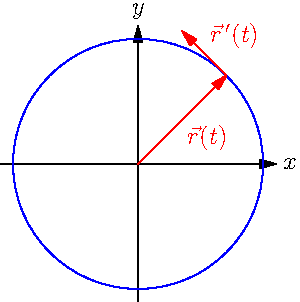
\includegraphics{./cap_curvas/pics/vetor_tangente_circunferencia}
\caption{O vetor tangente $\vct{r}\!~'(t)$}\label{circtang}
  \end{center}
\end{figure}


Observe que a norma do vetor tangente depende de como a curva é parametrizada e não apenas da curva em si. A fim de trabalhar com um objeto que independe da parametrização, é natural definirmos o vetor tangente unitário\index{vetor tangente unitário}, denotado por $\vct{T}$ (veja figura \ref{Frenet_Serret}):
\begin{equation}\label{defvecunit}
\|\vct{T}(t)\|=\frac{\vct{r}\!~'(t)}{\left\|\vct{r}\!~'(t)\right\|},\qquad \vct{r}\!~'(t)\neq \vct{0}.
\end{equation} 
A condição de existência para o vetor $\vct{T}$ é a função vetorial que parametriza a curva seja diferenciável que sua derivada seja diferente de zero, ou seja, que a parametrização seja regular.

\begin{obs} Quando $\vct{r}(t)$ representa a trajetória de uma partícula ao longo do tempo, a derivada $\vct{r}\!~(t)$ é a velocidade $\vct{v}(t)$ da partícula. Neste caso, o vetor tangente unitário é o versor associado a $\vct{v}(t)$:
$$\vct{v}(t)=v(t) \hat{v}(t)=v(t) \vct{T}(t).$$
A norma de $\vct{v}(t)$, denotada por $v(t)$, é chamada de velocidade escalar\index{velocidade escalar}. O vetor $\vct{T}(t)$ indica o sentido e a direção da velocidade.
\end{obs}

O vetor $\vct{T}$ pode ser definido de forma alternativa como segue: olhamos $s$ como função de $t$ na expressão (\ref{defcomparco_1}) e observamos que $s'(t)=\|\vct{r}\!~'(t)\|>0$. Assim, $s(t)$ é uma função contínua e monótona de $t$. Também, usando a rega da cadeia, temos:
$$
\frac{d\vct{r}}{dt}=\frac{d\vct{r}}{ds}\frac{ds}{dt}=\frac{d\vct{r}}{ds}\|\vct{r}\!~'(t)\|.
$$
Como $\vct{r}'(t)$ representa o vetor tangente, então
$$
\frac{d\vct{r}}{ds}=\frac{1}{\|\vct{r}\!~'(t)\|}\frac{d\vct{r}}{dt}=\vct{T}
$$
representa um vetor tangente unitário.

\begin{exer}
Considere as funções vetoriais dadas por
\begin{eqnarray*}
\vct{f}(t)&=&\cos(\pi t)\vct{i}+\sin(\pi t)\vct{j}\\
\vct{g}(t)&=&\cos(\pi t^3)\vct{i}+\sin(\pi t^3)\vct{j}
\end{eqnarray*}
Verifique que ambas parametrizam a mesma curva quando $-1\leq t \leq 1$. Verifique se as parametrizações são regulares e compare o comportamento da derivada em $t=0$. Que consequências isso tem para a existência do vetor tangente unitário? 
\end{exer}
% 
% \begin{wrapfigure}{r}{7cm}
% 
% 
% \begin{pspicture}(-3.5,-1.5)(2.5,4.0)
% 
% \psset{arrowscale=2,arrows=->,viewpoint=20 20 20,Decran=15,lightsrc=20 10 5}
% \defFunction[algebraic]%
% {helice}(t)
% {2*cos(2*t)}{5*sin(2*t)}{t}
% \psSolid[arrows=->,object=courbe,r=0,
% range=3 8,
% linecolor=blue,
% linewidth=0.05,
% resolution=360,
% function=helice]%
% 
%   \pstThreeDLine[linecolor=red,linewidth=1pt,arrows=->](1.9203406,-1.3970775,3.)(2.2653647,1.5669842,3.3087017)
%   \pstThreeDLine[linecolor=red,linewidth=1pt,arrows=->](1.9203406,-1.3970775,3.)(-1.0524784,-1.0330466,2.8272902)
%    \pstThreeDLine[linecolor=red,linewidth=1pt,arrows=->](1.9203406,-1.3970775,3.)(1.7122408,-1.6831192,5.9790728)
%       
%       
%  
%   \pstThreeDLine[linecolor=red,linewidth=1pt,arrows=->](-0.29,4.95,4)(-2.94,3.64,4.53)
%   \pstThreeDLine[linecolor=red,linewidth=1pt,arrows=->](-0.29,4.95,4)(0.6965073,2.1212711,3.7968617)
%   \pstThreeDLine[linecolor=red,linewidth=1pt,arrows=->](-0.29,4.95,4)(0.4292406,4.9891601,6.9119509)
%   
%   
%       
%   \pstThreeDLine[linecolor=red,linewidth=1pt,arrows=->](-1.6781431,-2.7201056,5. )(-0.9299871,-5.6049034,5.3438083)
%     \pstThreeDLine[linecolor=red,linewidth=1pt,arrows=->](-1.6781431,-2.7201056,5. )(1.1989964,-1.9351497,5.3254427)
%     \pstThreeDLine[linecolor=red,linewidth=1pt,arrows=->](-1.6781431,-2.7201056,5. )(-2.0810467,-2.471538,7.9624117)
%   
%   \pstThreeDLine[linecolor=red,linewidth=1pt,arrows=->](0.2734744,4.9530368,7.)(-2.4850089,5.9049461,7.6961596)
%     \pstThreeDLine[linecolor=red,linewidth=1pt,arrows=->](0.2734744,4.9530368,7.)(-0.6596792,2.1083429,7.1921997)
%   \pstThreeDLine[linecolor=red,linewidth=1pt,arrows=->](0.2734744,4.9530368,7.)(0.9945803,4.913222,9.9117728)
%   
%   \psPoint(-2.9,6.1,8){Nome1}
%       \rput*(Nome1){$\vct{T}$}
%   
%   \psPoint(-1,1.5,7.4){Nome2}
%       \rput*(Nome2){$\vct{N}$}
% 
%         \psPoint(1,5,10.4){Nome3}
%       \rput*(Nome3){$\vct{B}$}
% 
%   
%   
%   \axesIIID[linecolor=black](0,0,0)(4.5,4.5,11)
%  \end{pspicture}\caption{Triedro de Frenet-Serret}\label{Frenet_Serret}
%  
% \end{wrapfigure}
% 
% Agora, queremos definir um vetor ortogonal a $\vct{T}$ que esteja no mesmo plano formado por $\vct{r}'(t)$ e $\vct{r}''(t)$. Para isso, usamos o resultado do teorema \ref{teodernormacst}. Observe que a função vetorial $\vct{T}(t)$ possui módulo constante e, portanto, $\vct{T}(t)\cdot \vct{T}'(t)=0$. Observe que $\vct{T}(t)$ e $\vct{T}'(t)$ estão ambos no plano formado por $\vct{r}'(t)$ e $\vct{r}''(t)$ e são ortogonais entre si. No entanto, $\vct{T}'(t)$ não é necessariamente unitário. Logo, faz sentido definir o vetor normal unitário\index{vetor normal unitário} como
% $$
% \vct{N}=\frac{\vct{T}'(t)}{\|\vct{T}'(t)\|}.
% $$
% A figura \ref{Frenet_Serret} apresenta a representação de alguns vetores normais unitários.
% 
% Finalmente, vamos definir um vetor unitário que é simultanemente ortogonal a $\vct{T}$ e $\vct{N}$. A forma natural de obter um vetor ortogonal a outros dois vem do produto vetorial. Assim, o vetor binormal unitário\index{vetor binormal unitário} é definido como
% $$
% \vct{B}=\vct{T}\times\vct{N}.
% $$
% Das propriedades de produto vetorial, temos que $\vct{B}$, além de ortogonal a $\vct{T}$ e $\vct{N}$, é unitário e forma um sistema dextrogiro. O trio $\vct{T}$, $\vct{N}$ e $\vct{B}$ é chamado de triedro de Frenet-Serret. A figura \ref{Frenet_Serret} apresenta a representação de alguns triedros de Frenet-Serret.
% 
% 
% \section{Curvatura e Torção}
% 
% Nessa seção, estamos interessados em definir, a cada ponto da curva, funções que medem o quanto ela está torcida ou curvada, isto é, se a curva é muito diferente de uma reta ou se está fora de qualquer plano do espaço. Primeiro, definiremos uma função chamada de curvatura\index{curvatura}, que mede a cada ponto do domínio, a variação do vetor tangente com respeito ao comprimento de arco $s$. Naturalmente, queremos que a reta tenha curvatura nula, pois ela não difere da sua tangente em ponto algum. Para facilitar a visualização, podemos começar pensando apenas nas curvas que estão contidas em algum plano. A figura \ref{curvatura} nos dá uma ideia de curvatura.
% 
% \begin{figure}[!ht]
% \begin{center}
% \psset{xunit =1cm,yunit=1cm, linewidth=1\pslinewidth}
%  \begin{pspicture}(0,-1)(4,3)
%  
% \psplot[plotstyle=curve,linewidth=2\pslinewidth,linecolor=blue]{0}{3}{x}
% 
% \rput(1.5,-.5){Curvatura nula}
% 
% \end{pspicture}
%  \begin{pspicture}(0,-1)(4,3)
%  
% \psplot[plotstyle=curve,linewidth=2\pslinewidth,linecolor=blue]{0}{3}{x x mul 3 div}
% 
% \rput(1.5,-.5){Curvatura pequena}
% 
% \end{pspicture}
%  \begin{pspicture}(-2,-2)(2,2)
%  
% \parametricplot[plotstyle=curve,linewidth=2\pslinewidth,linecolor=blue]{0}{360}{3 t mul cos 2.718 -0.01 t mul exp mul 3 t mul sin 2.718 -0.01 t mul exp mul 2 mul}
% 
% \rput(0,-1.5){Curvatura grande}
% 
% \end{pspicture}
% 
% 
% \end{center}
% \caption{Ideia de curvatura.\label{curvatura}}
% \end{figure}
% 
% Pelo teorema \ref{teodernormacst}, temos que $\frac{d \vct{T} }{ds}$ é paralelo ao vetor normal $\vct{N}$, ou seja,
% \begin{equation}{\label{Frenet_1}}
% \frac{d \vct{T} }{ds}=\kappa   \vct{N},
% \end{equation}
% onde $\kappa(t)>0$ é uma função escalar chamada de curvatura. Por outro lado, calculamos a variação do vetor tangente com respeito ao comprimento de arco $s$ usando a regra da cadeia
% $$
% \frac{d \vct{T} }{ds}=\frac{d \vct{T} }{dt}\frac{dt}{ds}=\frac{d \vct{T} }{dt}\frac{1}{|s'(t)|},
% $$
% onde $s(t)$ é a função que mede o comprimento do arco dado pela expressão (\ref{defcomparco_1}). Usando o fato que $s'(t)=\|\vct{r}'(t)\|$, temos:
% $$
% \frac{d \vct{T} }{ds}=\frac{1}{\|\vct{r}'(t)\|}\frac{d \vct{T} }{dt}.
% $$
% Portanto, podemos escrever
% $$
% \kappa(t)=\frac{\|\vct{T}'(t)\|}{\|\vct{r}'(t)\|}.
% $$
% 
% Definimos também, para cada ponto $t$ do domínio, o raio de curvatura\index{raio de curvatura} $\rho(t)$ da forma:
% $$
% \rho(t)=\frac{1}{\kappa(t)}.
% $$
% O raio de curvatura tem a seguinte interpretação geométrica: considere um ponto $\vct{r}(t_0)$ onde da curvatura não é nula e defina o ponto $\vct{r}(t_0)+\kappa(t_0)\vct{N}$, chamado de centro de curvatura\index{centro de curvatura}. O círculo centrado no centro de curvatura e raio $\rho(t_0)$ é tangente a curva em $t_0$ e possui a mesma curvatura (veja a figura \ref{raio_de_curvatura}).
% 
% \begin{wrapfigure}{r}{9cm}
% 
% \begin{pspicture}(-6,-2)(3,7)
%   \psaxes{->}(0,0)(-5,-1)(2.5,6.5)        % sets up axis
% \psplot[plotstyle=curve,linewidth=2\pslinewidth,linecolor=blue]{-2}{2}{x x mul}
% 
% \parametricplot[algebraic=true,plotstyle=curve,linewidth=2\pslinewidth,linecolor=red]{-1}{.6}{-3.999848+5.59*cos(t),5.59*sin(t)+3.499924}
% 
% \rput(-4,3.2){Centro de curvatura}
%  \pscircle[algebraic=true,plotstyle=curve,linewidth=2\pslinewidth,linecolor=red](-3.999848,3.499924){.05}
% \end{pspicture}
% 
% \caption{Círculo de curvatura}\label{raio_de_curvatura}
% 
% \end{wrapfigure}
% \begin{exer}Calcule a curvatura da curva $\vct{r}=a\cos(t)\vct{i}+a\sin(t)\vct{j},\qquad a>0,\ 0\leq t\leq 2\pi$.
% \end{exer}
% \begin{ex}Dada a curva $y=x^2$, vamos encontrar a curvatura e o raio de curvatura no ponto $x=1$. Primeiro, encontramos uma parametrização para essa curva, por exemplo, $\vct{r}=t\vct{i}+t^2\vct{j}$. Calculamos:
% $$
% \vct{r}'=\vct{i}+2t\vct{j},
% $$
% $$
% \|\vct{r}'\|=\sqrt{1+4t^2},
% $$
% $$
% \vct{T}=\frac{1}{\sqrt{1+4t^2}}\left(\vct{i}+2t\vct{j}\right)
% $$
% e
% $$
% \vct{T}'=-\frac{4t}{\sqrt{(1+4t^2})^3}\vct{i}+\left(-\frac{8t^2}{\sqrt{(1+4t^2})^3}+\frac{2}{\sqrt{1+4t^2}}\right)\vct{j},
% $$
% Em $t=1$, temos:
% $$
% \|\vct{r}'\|=\sqrt{5},
% $$
% $$
% \vct{T}'=-\frac{4}{\sqrt{5^3}}\vct{i}+\left(-\frac{8}{\sqrt{5^3}}+\frac{2}{\sqrt{5}}\right)\vct{j}=-\frac{4}{\sqrt{5^3}}\vct{i}+\frac{2}{\sqrt{5^3}}\vct{j},
% $$
% e
% $$
% \|\vct{T}'\|=\sqrt{\frac{16}{5^3}+\frac{4}{5^3}}=\frac{2}{5}.
% $$
% Portanto,
% $$
% \kappa(1)=\frac{\|\vct{T}'\|}{\|\vct{r}'\|}=\frac{2}{5\sqrt{5}}
% $$
% e
% $$
% \rho(1)=\frac{5\sqrt{5}}{2}.
% $$
% veja representação geométrica na figura \ref{raio_de_curvatura}.
% \end{ex}
% 
% O leitor deve ter observado que conhecendo somente a curvatura não é possível reconstruir uma curva a partir de um ponto dado. Um curva pode não estar contida em plano algum no espaço e, por isso, precisamos definir uma função escalar, chamada torção, que mede a magnitude da variação do vetor binormal. A figura \ref{torcao} apresenta uma ideia de torção\index{torção}: uma curva contida em algum plano no espaço tem torção nula e quando maior a variação com respeito ao plano definido por $\vct{T}$ e $\vct{N}$, maior a torção. O leitor deve tomar cuidado na interpretação da figura \ref{torcao}, pois se esticarmos indefinidamente a hélice circular representada, ela voltará a se aproximar de uma reta, que tem torção nula (veja problema \ref{prob_torcao}). Sabendo que a torção será definida em termos da variação do vetor binormal com respeito ao comprimento de arco $s(t)$, fazendo algumas observações:
% $$
% \frac{d\vct{B}}{ds}=\frac{d}{ds}\left(\vct{T}\times\vct{N}\right)=\frac{d\vct{T}}{ds}\times \vct{N}+\vct{T}\times\frac{d\vct{N}}{ds}.
% $$
% Usando a expressão (\ref{Frenet_1}), temos que $\frac{d\vct{T}}{ds}=\kappa\vct{N}$, logo 
% $$
% \frac{d\vct{B}}{ds}=\vct{T}\times\frac{d\vct{N}}{ds}.
% $$
% Isso implica que $\frac{d\vct{B}}{ds}$ é ortogonal a $\vct{T}$. Mas, pelo teorema \ref{teodernormacst}, temos que $\frac{d\vct{B}}{ds}$ é ortogonal a $\vct{B}$. Logo, $\frac{d\vct{B}}{ds}$ é paralelo a $\vct{N}$, ou seja,
% \begin{equation}{\label{Frenet_2}}
% \frac{d\vct{B}}{ds}=-\tau\vct{N},
% \end{equation}
% onde $\tau$ é chamado de torção\index{torção}. O sinal negativo tem um propósito: quando $\tau>0$, $\frac{d\vct{B}}{ds}$ está no sentido de $-\vct{N}$; então se $P$ é um ponto sobre a curva movendo-se no sentido positivo, $\vct{B}$ gira em torno de $\vct{T}$ como um parafuso de rosca direita sendo apertado (veja a figura \ref{Curvatura_torcao_1}). Em alguns contextos, calculamos a módulo da torção, dada por
% $$
% |\tau|=\left\|\frac{d\vct{B}}{ds}\right\|=\frac{\|\vct{B}'(t)\|}{\|\vct{r}'(t)\|}.
% $$
% 
% \begin{figure}[!ht]
% \begin{center}
% \psset{xunit =1cm,yunit=1cm, linewidth=1\pslinewidth}
% \begin{pspicture}(-2.5,-2.0)(2.5,4.0)
% \psset{viewpoint=20 20 20,Decran=15,lightsrc=20 10 5}
% \defFunction[algebraic]%
% {helice}(t)
% {2*cos(2*t)}{5*sin(2*t)}{0}
% \psSolid[arrows=->,object=courbe,r=0,
% range=0 5,
% linecolor=blue,
% linewidth=0.05,
% resolution=360,
% function=helice]%
% \rput(1.0,-1.8){Torção nula}
%   \axesIIID[linecolor=black](0,0,0)(4.5,6,5)
% \end{pspicture}
% \begin{pspicture}(-2.5,-2.0)(2.5,4.0)
% \psset{viewpoint=20 20 20,Decran=15,lightsrc=20 10 5}
% \defFunction[algebraic]%
% {helice}(t)
% {2*cos(2*t)}{5*sin(2*t)}{t/4}
% \psSolid[arrows=->,object=courbe,r=0,
% range=0 4,
% linecolor=blue,
% linewidth=0.05,
% resolution=360,
% function=helice]%
% \rput(1.0,-1.8){Torção pequena}
%   \axesIIID[linecolor=black](0,0,0)(4.5,6,5)
% \end{pspicture}
% \begin{pspicture}(-2.5,-2.0)(2.5,4.0)
% \psset{viewpoint=20 20 20,Decran=15,lightsrc=20 10 5}
% \defFunction[algebraic]%
% {helice}(t)
% {2*cos(2*t)}{5*sin(2*t)}{2*t}
% \psSolid[arrows=->,object=courbe,r=0,
% range=0 4,
% linecolor=blue,
% linewidth=0.05,
% resolution=360,
% function=helice]%
% \rput(1.0,-1.8){Torção grande}
%   \axesIIID[linecolor=black](0,0,0)(4.5,6,7)
% \end{pspicture}
% 
% \end{center}
% \caption{Ideia de torção.\label{torcao}}
% \end{figure}
% Ainda, definimos o raio de torção\index{raio de torção} por
% $$
% \sigma(t)=\frac{1}{\tau(t)}.
% $$
% 
% Podemos calcular $\frac{d\vct{N}}{ds}$ em termos da curvatura e da torção:
% \begin{equation*}
% \frac{d\vct{N}}{ds}=\frac{d}{ds}\left(\vct{B}\times\vct{T}\right)=\frac{d\vct{B}}{ds}\times \vct{T}+\vct{B}\times\frac{d\vct{T}}{ds}.
% \end{equation*}
% Usando as expressões (\ref{Frenet_1}) e (\ref{Frenet_2}), escrevemos
% \begin{equation*}
% \frac{d\vct{N}}{ds}=-\tau\vct{N} \times \vct{T}+\vct{B}\times \kappa \vct{N}.
% \end{equation*}
% ou seja,
% \begin{equation}{\label{Frenet_3}}
% \frac{d\vct{N}}{ds}=-\kappa \vct{T}+\tau \vct{B}.
% \end{equation}
% As equações (\ref{Frenet_1}), (\ref{Frenet_2}) e (\ref{Frenet_3}) são chamadas de Fórmulas de Frenet-Serret.
% 
% Como esperávamos, se $\kappa=0$, então $\frac{d\vct{T}}{ds}=\vct{0}$, o que implica que $\vct{T}$ não varia ao longo da curva, ou seja, a curva é uma reta. Agora, se $\tau=0$, então $\frac{d\vct{B}}{ds}=\vct{0}$ e $\vct{B}$ é um vetor constante. Como $\vct{B}\cdot \vct{T}=\vct{B}\cdot \frac{d\vct{r}}{ds}=0$, então podemos integrar para obter $\vct{B}\cdot (\vct{r}-\vct{r_0})=0$, onde $r_0$ é um vetor constante da integração. Logo $\vct{r}$ está contido no plano ortogonal a $\vct{B}$.
% 
% 
% 
% \begin{ex} Vamos calcular curvatura, raio de curvatura e o módulo da torção para a hélice circular $\vct{r}(t)=\cos(t)\vct{i}+\sin(t)+t\vct{k}$:
% $$
% \vct{r}'(t)=-\sin(t)\vct{i}+\cos(t)+\vct{k},
% $$
% $$
% \|\vct{r}'(t)\|=\sqrt{2},
% $$
% $$
% \vct{T}(t)=-\frac{\sin(t)}{\sqrt{2}}\vct{i}+\frac{\cos(t)}{\sqrt{2}}+\frac{1}{\sqrt{2}}\vct{k},
% $$
% $$
% \vct{T}'(t)=-\frac{\cos(t)}{\sqrt{2}}\vct{i}-\frac{\sin(t)}{\sqrt{2}},
% $$
% $$
% \|\vct{T}'(t)\|=\frac{1}{\sqrt{2}},
% $$
% $$
% \kappa(t)=\frac{1}{\sqrt{2}}\cdot \frac{1}{\sqrt{2}}=\frac{1}{2},
% $$
% $$
% \rho(t)=2,
% $$
% $$
% \vct{N}(t)=-\cos(t)\vct{i}-\sin(t)\vct{j},
% $$
% \begin{eqnarray*}
% \vct{B}(t)&=&\left|\begin{array}{ccc}\vct{i}&\vct{j}&\vct{k}\\-\frac{\sin(t)}{\sqrt{2}}&\frac{\cos(t)}{\sqrt{2}}&\frac{1}{\sqrt{2}}\\-\cos(t)&-\sin(t)&0\end{array}\right|\\
% &=&\frac{\sin(t)}{\sqrt{2}}\vct{i}-\frac{\cos(t)}{\sqrt{2}}\vct{j}+\frac{1}{\sqrt{2}}\vct{k}.
% \end{eqnarray*}
% $$
% \vct{B}'(t)=\frac{\cos(t)}{\sqrt{2}}\vct{i}+\frac{\sin(t)}{\sqrt{2}}\vct{j},
% $$
% $$
% \|\vct{B}'(t)\|=\frac{1}{\sqrt{2}},
% $$
% $$
% |\tau(t)|=\frac{1}{2}.
% $$
% \end{ex}
% 
% \begin{exer} Calcule a curvatura, o raio de curvatura e o módulo da torção das curvas abaixo:
% \begin{itemize}
% \item[a)] $\vct{r}=a\cosh(t)\vct{i}+b\sinh(t)\vct{j}$, $-\infty<t<\infty$, $a>0,\ b>0$.
% \item[b)] $\vct{r}=a\cos(t)\vct{i}+b\sin(t)\vct{k}$, $0\leq t\leq 2\pi$, $a>0,\ b>0$.
% \item[c)] $\vct{r}=a\cos(t)\vct{i}+a\sin(t)+ct\vct{k}$, $t\geq 0$, $a>0,\ c>0$.
% 
% \end{itemize}
% \end{exer}
% 
% \begin{exer}{\label{prob_torcao}} Dada a hélice circular $\vct{r}=a\cos(t)\vct{i}+a\sin(t)+ct\vct{k}$, $t\geq 0$, $a>0,\ c>0$, calcule o valor de $c$ para que a torção seja máxima.
% \end{exer}
% 
% \begin{wrapfigure}{r}{8cm}
% \begin{pspicture}(-1.0,2)(6.5,8.0)
% 
% \psset{arrowscale=2,arrows=->,viewpoint=12 12 12,Decran=15,lightsrc=20 10 5}
% \defFunction[algebraic]%
% {helice}(t)
% {2*cos(2*t)}{5*sin(2*t)}{t}
% \psSolid[arrows=->,object=courbe,r=0,
% range=6.5 8,
% linecolor=blue,
% linewidth=0.05,
% resolution=360,
% function=helice]%
%        
%   \pstThreeDLine[linecolor=red,linewidth=1pt,arrows=->](0.2734744,4.9530368,7.)(-2.4850089,5.9049461,7.6961596)
%     \pstThreeDLine[linecolor=red,linewidth=1pt,arrows=->](0.2734744,4.9530368,7.)(-0.6596792,2.1083429,7.1921997)
%     \pstThreeDLine[linecolor=green,linewidth=1pt,arrows=->](0.2734744,4.9530368,7.)(1.206628,7.7977307,6.8078003)
%     
%   \pstThreeDLine[linecolor=red,linewidth=1pt,arrows=->](0.2734744,4.9530368,7.)(0.9945803,4.913222,9.9117728)
%   %\pstThreeDCoor[IIIDticks]
%   \pstThreeDEllipse[beginAngle=0,endAngle=90,linestyle=dashed](0.27,5,7.)(-2.55,1.4,0.6)(0.1,-2.0,0.19)
%     \pstThreeDEllipse[beginAngle=0,endAngle=90,linestyle=dashed](0.4,6.2,8.5)(0.7211059,0.0,2.911772)(0.9,3.5,-1.2)
%     
%  %    \pstThreeDLine[linecolor=green,linewidth=1pt,arrows=->](0,0,0)(3,0,0)
%   %  \pstThreeDEllipse[beginAngle=0,endAngle=90](0,0,0)(3,0,0)(0,3,0)
%   
%   \psPoint(-2.9,6.0,7.2){Nome1}
%       \rput*(Nome1){$\vct{T}$}
%   
%   \psPoint(-1,1.5,7.3){Nome2}
%       \rput*(Nome2){$\vct{N}$}
% 
%         \psPoint(1.5,8.2,6.8){Nome2a}
%       \rput*(Nome2a){$-\vct{N}$}
% 
%       
%         \psPoint(1,5,10.2){Nome3}
%       \rput*(Nome3){$\vct{B}$}
% 
%       
%               \psPoint(-2.4,5.5,8.0){Nome4}
%       \rput*(Nome4){Curvatura}
% 
%               \psPoint(1.5,7.5,7.5){Nome5}
%       \rput*(Nome5){Torção}
% 
%       \psPoint(3.5,4,7.1){Nome6}
%       \rput*(Nome6){$\vct{r}(t)$}
%       
% %  \axesIIID[linecolor=black](0,0,0)(4.5,4.5,11)
%  \end{pspicture}\caption{Curvatura e Torção}\label{Curvatura_torcao_1}
%  
% \end{wrapfigure}
% 
% A curvatura e a torção podem ser calculadas de maneira mais simples. Para concluir isso, começamos calculando as derivadas de $\vct{r}$. Usamos aqui que $s'(t)=\|\vct{r}'(t)\|$, obtida da equação (\ref{defcomparco_1}):
% $$
% \vct{r}'=\frac{d\vct{r}}{ds}\frac{ds}{dt}=s' \vct{T},
% $$
% \begin{eqnarray*}
% \vct{r}''&=&s'' \vct{T}+s' \vct{T}'\\&=&s'' \vct{T}+s' \|\vct{T}'\|\vct{N}\\
% &=&s'' \vct{T}+s'^2 \kappa \vct{N}
% \end{eqnarray*}
% e
% \begin{eqnarray*}
% \vct{r}'''&=&s''' \vct{T}+s''\vct{T}'+2s's''\kappa \vct{N}+s'^2 \left(\kappa \vct{N}'+\kappa' \vct{N}\right)\\
% &=&s''' \vct{T}+s''s'\kappa \vct{N}+\left(2s's''\kappa+s'^2\kappa'\right) \vct{N}\\
% &+&s'^3 \kappa (-\kappa \vct{T}+\tau\vct{B})\\
% &=&\left(s'''-\kappa^2s'^3\right) \vct{T}+\left(3s''s'\kappa +s'^2\kappa'\right)\vct{N}+s'^3 \kappa \tau\vct{B},
% \end{eqnarray*}
% onde usamos as expressões (\ref{Frenet_1}) e (\ref{Frenet_3}). Agora, tomamos os seguintes produtos:
% $$
% \vct{r}'\times \vct{r}''=s'^3\kappa \vct{B}\qquad\text{e}\qquad
% \vct{r}'\times \vct{r}''\cdot \vct{r}'''=s'^6\kappa^2\tau.
% $$
% Isso implica em 
% $$
% \|\vct{r}'\times \vct{r}''\|=|s'|^3\kappa\qquad\text{e}\qquad
% \vct{r}'\times \vct{r}''\cdot \vct{r}'''=\|\vct{r}'\times \vct{r}''\|^2\tau.
% $$
% ou seja,
% \begin{equation}{\label{curvatura_2}}
% \kappa =\frac{\|\vct{r}'\times \vct{r}''\|}{\|r'\|^3}
% \end{equation}
% e
% \begin{equation}{\label{torcao_2}}
% \tau=\frac{\vct{r}'\times \vct{r}''\cdot \vct{r}'''}{\|\vct{r}'\times \vct{r}''\|^2}.
% \end{equation}
% 
% \begin{obs}Uma aplicação natural é a decomposição da aceleração em suas componentes tangencial e normal. Observe que
% $$
% \vct{r}'=\vct{v}=v\vct{T}=s' \vct{T}
% $$
% e
% $$
% \vct{a}=v' \vct{T}+v^2 \kappa \vct{N}.
% $$
% Concluímos que a aceleração está no plano normal a $\vct{B}$ e possui componentes tangencial e normal:
% $$
% \vct{a}=a_T \vct{T}+a_N \vct{N},
% $$
% onde $a_T=v'$ e $a_N=v^2\kappa$. Então, se a velocidade possui normal constante, temos que $v'=0$ e a aceleração possui apenas componente normal.
% 
% \end{obs}
% \begin{exer}Calcule curvatura e torção para a curva $\vct{r}=a\cos(t)\vct{i}+a\sin(t)\vct{j}+ct\vct{k}$, $a>0$, $c>0$, $t>0$ usando as expressões (\ref{curvatura_2}) e (\ref{torcao_2}).
% \end{exer}
% 
% \begin{ex}Uma motocicleta percorre uma trajetória circular de raio $20m$ com velocidade constante em módulo. A motocicleta poderá derrapar se a aceleração normal exceder $2m/s^2$. Qual é a velocidade máxima do motocicleta para que ela não derrape?
% \end{ex}
% 
% \begin{ex} Consideremos agora, a curva gerada pelas seguintes equações paramétricas:
% $$x(t)=\cos(t)\qquad y(t)=\sin(t)\qquad z(t)=f(t).$$
%  Onde $f(t)$ é uma função dada. Observe que a projeção desta curva no plano $xy$ é uma circuferência de raio 1. A curva é, portanto, gerada pela trajetória de ponto cuja projeção do movimento no plano $xy$ é cirvular e a altura é dada pela função $f(t)$. Podemos calcular a curvatura e a torção conforme a seguir:
%  \begin{eqnarray*}
%   \vec{r}(t)&=&\cos(t)\vec{i}+\sin(t)\vec{j}+f(t)\vec{k}\\
%   \vec{r'}(t)&=&-\sin(t)\vec{i}+\cos(t)\vec{j}+f'(t)\vec{k}\\
%   \vec{r''}(t)&=&-\cos(t)\vec{i}-\sin(t)\vec{j}+f''(t)\vec{k}\\
%   \vec{r'''}(t)&=&\sin(t)\vec{i}-\cos(t)\vec{j}+f'''(t)\vec{k}
%  \end{eqnarray*}
% Assim, calculamos:
%  \begin{eqnarray*}
%   \vec{r'}(t)\times\vec{r''}(t) &=&\left[f''(t)\cos(t)+f'(t)\sin(t)\right]\vec{i}+\left[-f'(t)\cos(t)+f''(t)\sin(t)\right]\vec{j}+\vec{k}\\
%  \vec{r'}(t)\times\vec{r''}(t)\cdot r'''(t)&=&f'(t)+f'''(t)\\
%  \|\vec{r'}(t)\times\vec{r''}(t)\|&=&\sqrt{1+\left(f'(t)\right)^2+\left(f''(t)\right)^2}\\
%  \|\vec{r'}(t)\|&=&\sqrt{1+\left(f'(t)\right)^2}
%  \end{eqnarray*}
% E finalmente, obtemos:
%  \begin{eqnarray*}
% \kappa&=&\frac{\sqrt{1+\left(f'(t)\right)^2+\left(f''(t)\right)^2}}{\left({1+\left(f'(t)\right)^2}\right)^{3/2}}\\
% \tau&=&\frac{f'(t)+f'''(t)}{1+\left(f'(t)\right)^2+\left(f''(t)\right)^2}
%  \end{eqnarray*}
% Podemos, agora, explorar diversos casos particular:
% \begin{itemize}
%  \item [a)] Caso $f(t)=c$ constante. Neste caso, recaímos na circunferência de raio 1, cuja curvatura é 1 e a torção é nula.
%  \item [b)] Caso $f(t)=ct$ com $c$ constante. Recaímos na hélice cicular uniforme, já estudada, cuja curvatura é $\frac{1}{1+c^2}$ e a torção é $\frac{c}{1+c^2}$.
%  \item [c)] Caso $f(t)=ct^2$ com $c$ constante. Recaímos na hélice cicular com espaçamento linearmente crescente, cuja curvatura é dada por ${\frac {\sqrt {4\,{c}^{2}+1+4\,{c}^{2}{t}^{2}}}{ \left( 1+4\,{c}^{2}{t
% }^{2} \right) ^{3/2}}}$ e cuja torção é dada por $2\,{\frac {ct}{4\,{c}^{2}+1+4\,{c}^{2}{t}^{2}}}$.
%  \item [d)] Caso $f(t)=\sin(t)$. Recaímos na elipse de semieixos $1$ e $\sqrt{2}$ no plano $y=z$. Neste caso, a curvatura é $\kappa=\frac{\sqrt{2}}{\left(1+\cos(t)^2\right)^{3/2}}$ e a torção é nula.
%  \item [e)] Caso $\tau=0$, isto é, $f'(t)+f'''(t)=0$, o que é equivalente a $f(t)=a+b\cos(t)+c\sin(t)$ onde $a$, $b$ e $c$ são constantes. Recaímos na elipse de semieixos $1$ e $\sqrt{1+b^2+c^2}$ no plano $z=bx+cy$. Neste caso, a curvatura é $\kappa={\frac {\sqrt {b^2+c^2+1}}{\left(1-bc\sin(2t)+c^2\cos^2(t)+b^2\sin^2(t) \right) ^{3/2}}}$ e a torção é nula.
%   \end{itemize}
% 
%  
%  
% \end{ex}
% 
% 
% 
% 
% 
%\end{document}